
\chapter{Analyse de l'existant}


Le domaine de la vérification et de la validation regroupe un ensemble de
techniques du cycle de développement des logiciels qui ont pour objectif de
s'assurer de leur correction et de leur sûreté. Ces deux notions sont apparues
dans les années soixante-dix avec les travaux de \bsc{Dijkstra} \cite{Dijkstra},
\bsc{Floyd} \cite{Floyd} et \bsc{Hoare} \cite{Hoare}.

La correction d'un logiciel représente le respect de l'implémentation par
rapport aux spécifications. La sûreté d'un logiciel est liée à son absence
d'erreurs à l'exécution.


\section{Model-checking}
\label{sec:model-checking}

Le model-checking \cite{model-checking} permet de vérifier algorithmiquement si
un modèle donné (le système ou une abstraction de ce système) satisfait une
spécification, formulée en termes de logique temporelle \cite{LTL}. Un modèle
est un ensemble d'états, de propriétés que vérifie chaque état, et de
transitions entre ces états qui décrivent l'évolution du système.\\

Le model-checking couvre l'ensemble des états du système et des transitions afin
d'analyser toutes les exécutions possibles du système. Sur de grands systèmes,
cette méthode est pénalisée par l'explosion combinatoire du nombre des états (et
la complexité en temps ou en espace qui en résulte). Il est néanmoins possible
de modéliser des algorithmes asynchrones répartis et des automates non
déterministes, comme le fait notamment l'outil \textsc{Spin} \cite{SPIN}.\\

La plateforme \textsc{Frama-C} du LSL intègre \textsc{Aoraï}, un greffon
permettant d'annoter automatiquement le code source d'un programme C d'après
une formule de logique temporelle linéaire, de sorte que les annotations sont
vérifiées si le programme repecte la formule.


\section{Analyse statique}
\label{sec:AS}

L'analyse statique \cite{static-analysis} examine le code source du programme
sans l'exécuter. Elle raisonne sur tous les comportements qui pourraient
survenir lors de l'exécution et permet donc de déduire des propriétés devant
être vérifiées pour toutes ces exécutions, dans le but de prouver la correction
du programme.\\

En revanche, la vérification de programme étant en général indécidable
\cite{undecidability}, il est souvent nécessaire d'utiliser des
sur-approximations, ce qui implique que les résultats peuvent être moins précis
que ce que l'on souhaite mais ils sont garantis pour toutes les exécutions.
Ainsi, on peut établir des propriétés de sûreté ({\em safety}), où l’on cherche
des invariants sur les valeurs des variables du programme (une plage de valeurs
par exemple), afin d'exclure certains risques d'erreurs à l'exécution.\\

Parmi les méthodes statiques sont distinguées : l'interprétation abstraite
(section~\ref{sec:interpretation-abstraite}), l'abstraction à partir de
prédicats (section~\ref{sec:abstraction-predicats}) et la preuve de théorèmes
(section~\ref{sec:preuve}).



\subsection{\textsc{Frama-C} et \textsc{Acsl}}
\label{sec:frama-c}

\textsc{Frama-C} \cite{Frama-C} est une plate-forme dédiée à l'analyse statique
des programmes C, conjointement dévelopée par INRIA et le CEA LIST. Son
architecture (Fig.~\ref{fig:archi}) comporte un noyau et un écosystème de
greffons, rendant l’outil extensible. Les greffons peuvent échanger des
informations et utiliser les  services fournis par le noyau, permettant ainsi
une collaboration entre différentes analyses.\\


\newcommand{\lang}[1]{\textsf{\small #1}\xspace}
\newcommand{\cil}{\lang{CIL}}
\newcommand{\C}{\lang{C}}
\newcommand{\ACSL}{\lang{ACSL}}
\newcommand{\JML}{\lang{JML}}
\newcommand{\framac}{\lang{Frama-C}}
\newcommand{\pathcrawler}{\lang{PathCrawler}}
\newcommand{\colibri}{\lang{Colibri}}


\begin{figure}[h]
  \begin{center}
  \tikzstyle{service}=
            [rounded corners,rectangle,draw,inner sep=2mm,fill=gray!40]
  \pgfdeclarelayer{db-background}
  \pgfdeclarelayer{background}
  \pgfsetlayers{background,db-background,main}
  \scalebox{0.75}{
    \begin{tikzpicture}
      \node at (0,5.5) { \large{\textbf{Plug-ins}} };
      \node [matrix of nodes,rectangle,draw,column sep=4mm,inner sep=2.5mm] 
      (analyzers) at (8,5.5)
            {
              \node [service] (a1) at (0,0) { Analyzer 1 }; \pgfmatrixnextcell
              \node [service] (a2) at (0,0) { Analyzer 2 }; \pgfmatrixnextcell
              \node [service] (a3) at (0,0) { Analyzer 3 }; \pgfmatrixnextcell
              \node [service] (a5) at (0,0) { \vphantom{Analyzer} \ldots }; \\
            };
            \node[inner sep=0.4mm] (db-plugins) at (8,3.7) {Plug-ins Database };
            \node[] (db-kernel) at (db-plugins) {};
            \begin{pgfonlayer}{db-background}
              \node[service,ellipse,fit=(db-plugins)
                (db-kernel),inner sep=1.2mm] (db) {};
            \end{pgfonlayer}
            \node at (0,2.35) { \large{\textbf{Kernel Services}} };
            \begin{pgfonlayer}{background}
              \node [matrix of nodes,rectangle,draw,row sep=4mm,inner sep=2mm] 
              (services) at  (8,2.35)
                    {
                      \node [inner sep=6mm] at (0,0) {};
                      \node [service] (message) at (0,-0.3) { Message };
                      \pgfmatrixnextcell
                      \node [service] (printer) at (0,-0.3) { Printer };
                      \pgfmatrixnextcell
                      \node [service] (status) at (0,-0.3) { Property Status };
                      \pgfmatrixnextcell \\
                      \node [service] (journal) at (1,0) { Journal };
                      \pgfmatrixnextcell
                      \node [service] (parameter) at (1,0) { Parameter };
                      \pgfmatrixnextcell
                      \node [service] (project) at (0.1,0) { Project };
                      \pgfmatrixnextcell 
                      \node [service] (others) at (0.1,0)
                            { \vphantom{Project} \dots}; \pgfmatrixnextcell\\
                    };
      \end{pgfonlayer}
            \node at (0,-0.2) { \large{\textbf{(Modified) \cil}} };
            \node [service,diamond,aspect=3,inner sep=1mm] (ast) at (8,-0.2)
                  { C + \textsc{Acsl} AST };
            \path [->,thick] (5,3.73) edge[bend left=30] (5,4.87);
            \path [->,thick] (11.5,3.73) edge[bend right=30] (11.5,4.87);
            \path [->,thick] (analyzers) edge (db);
            \path [<->,thick] (ast) edge (services);
    \end{tikzpicture}
  }
  \end{center}
  \caption{Architecture de \textsc{Frama-C}}\label{fig:archi}
\end{figure}


\textsc{Frama-C} est basé sur CIL \cite{CIL}, une bibliothèque qui normalise des
programmes C (ISO C99) en opérant des modifications syntaxiques : normalisation
des boucles en utilisant la structure ${\tt while}$, unique ${\tt return}$ pour
chaque fonction, etc. \textsc{Frama-C} étend CIL pour supporter des annotations
dédiées portant sur le code source, exprimées dans le langage \textsc{Acsl}.
\textsc{Acsl} \cite{ACSL} est un langage formel de spécification
comportementale \cite{BISL}, inspiré de JML \cite{JML}, pouvant exprimer des
propriétés fonctionnelles de programmes C : pré-conditions, post-conditions,
invariants, etc.\\

En effet, la spécification d'une fonction comprend les pré-conditions requises
(exprimées par une clause ${\tt requires}$) lors de l'appel et les
post-conditions assurées (${\tt ensures}$) lors du retour. Parmi ces
post-conditions, une clause indique quels sont les emplacements mémoire qui
peuvent être affectés (${\tt assigns}$) par la fonction.\\


\begin{figure}[h]
\begin{lstlisting}
/*@ requires \valid(a) && \valid(b);
    requires \separated(a,b);
    assigns *a, *b;
    ensures *a == \at(*b,Pre);
    ensures *b == \at(*a,Pre); */
void swap(int* a, int* b);
\end{lstlisting}
\caption{Exemple de spécification \textsc{Acsl}}\label{fig:acsl-spec}
\end{figure}


Considérons par exemple une spécification fournie pour une fonction $swap$
(Fig.~\ref{fig:acsl-spec}). La première pré-condition établit que les deux
arguments doivent être des pointeurs valides, autrement dit, le déréférencement
de $a$ ou de $b$ ne produira pas d'erreur à l'exécution. La seconde
pré-condition impose que les emplacements mémoire occupés par chacune de ces
variables soient disjoints. En plus de ${\tt \backslash valid}$ et
${\tt \backslash separated}$, \textsc{Acsl} fournit de nombreux prédicats et
fonctions afin de décrire les états de la mémoire. ${\tt \backslash at(e,l)}$
fait référence à la valeur de l'expression $e$ à l'état de la mémoire au label
$l$. $Pre$ est un label prédéfini qui fait référence à l'état de la mémoire
avant l'exécution de la fonction. Ainsi, les post-conditions (${\tt ensures}$)
signifient qu'à la fin de la fonction, $*a$ aura la valeur que $*b$ avait au
début de la fonction, et réciproquement.\\


\textsc{Acsl} offre aussi la possibilité d'écrire des annotations dans le code
source, permettant d'exprimer des propriétés devant être vraies à un point donné
du programme : les assertions (${\tt assert}$).
Il est également possible d'exprimer des propriétés devant être vraies avant une
boucle et après chaque itération de cette boucle : les invariants de boucle
(${\tt loop\ invariant}$).\\


Les annotations du langage \textsc{Acsl} sont écrites en utilisant la logique
du premier ordre, et il est possible de définir ses propres fonctions et
prédicats.
Les greffons peuvent valider ou invalider les propriétés \textsc{Acsl} et
générer des annotations \textsc{Acsl}, les annotations sont donc un moyen
d'échanger des informations entre les différentes analyses opérées par les
greffons.


\subsection{Interprétation abstraite}
\label{sec:interpretation-abstraite}

L'interprétation abstraite \cite{abstract-interpretation} s'appuie sur les
théories du point-fixe et des domaines pour introduire des sur-approximations
des comportements d'un programme. Elle consiste à abstraire les domaines des
variables par des domaines finis et beaucoup plus petits. Par exemple, le
domaine des entiers pourrait être abstrait par un domaine de trois valeurs :
$(-, 0, +)$. Appliquée à l’analyse de valeurs, elle consiste à calculer à
chaque ligne du code une sur-approximation de l’ensemble des valeurs prises par
chaque variable en cette ligne lors de toutes les exécutions du programme,
permettant ainsi de détecter certaines erreurs comme les divisions par zéro ou
les accès en dehors des bornes des tableaux.\\

Pour contourner le problème d’indécidabilité, la théorie de l’interprétation
abstraite construit une méthode qui, à la même question, répondra ``oui'',
``non'' ou ``peut-être''. Si la méthode répond ``peut-être'', c’est qu’on n’a pu
prouver ni l’un ni l’autre des deux premiers cas. C’est ce qu’on appelle une
alarme : il est possible qu’une des exécutions du programme produise une erreur
donnée, mais nous n’avons été capable ni de le confirmer ni de l’infirmer.
L’erreur signalée par une alarme peut ne jamais apparaître à l’exécution, dans
ce cas on l’appelle fausse alarme. On ne calcule donc pas la propriété exacte
mais une abstraction de cette propriété, en imposant la contrainte de sûreté
suivante : ``la propriété abstraite calculée ne doit oublier aucune exécution
concrète''. L'abstraction est effectuée à partir de prédicats atomiques
définissant des abstractions des domaines des variables.\\

\textsc{PolySpace C Verifier} \cite{PolySpace} a été le premier outil commercial
utilisant l'interprétation abstraite pour détecter les erreurs à l'exécution
dans les programmes en C, C++ et Ada mais signale beaucoup de fausses alarmes.
L'ENS a développé \textsc{Astrée} \cite{ASTREE}, spécifique au langage C et aux
logiciels critiques. Le CEA LIST a développé \textsc{Fluctuat} \cite{Fluctuat},
qui mesure précisément les approximations faites à l'exécution d'un programme C.
\textsc{Frama-C} intègre un greffon d'interprétation abstraite : \textsc{Value}
\cite{Value}.



\subsection{Abstraction à partir de prédicats}
\label{sec:abstraction-predicats}

L'abstraction à partir de prédicats \cite{predicate-abstraction} est une
technique permettant de générer automatiquement des abstractions de systèmes au
nombre d'états infini. Pour un programme $P$ au nombre d'états infini, un
ensemble fini de prédicats $E = \{f_1, ..., f_n\}$ est défini, ces prédicats
sont des expressions booléennes sur les variables de $P$ et les constantes du
langage.\\

Chaque état concret de $P$ est mis en correspondance avec un état abstrait de
l'abstraction de $P$, après évaluation par les prédicats de $E$. Un état
abstrait est un $n$-upplet de valeurs booléennes correspondant à la
satisfaisabilité des $n$ prédicats (au moyen d'un solveur SMT).\\

Par exemple, si 3 prédicats $f_1, f_2, f_3$ sont définis et que la
satisfaisabilité de ces prédicats à l'état concret $e$ est évaluée
respectivement à $false, true, true$, alors dans l'abstraction générée, l'état
$e$ correspond à l'état abstrait $(\lnot f_1, f_2, f_3)$.\\

L'abstraction générée comporte un nombre fini d'états (au plus $2^n$) car il n'y
a qu'un nombre fini de prédicats, le model-checking peut donc être appliqué à
cette abstraction. Si une propriété de sûreté est vérifiée dans l'abstraction,
elle l'est également dans le système concret.

Cette technique est notamment utilisée par l'outil \textsc{Slam} \cite{SLAM} de
Microsoft.


\subsection{Preuve de théorèmes}
\label{sec:preuve}

La preuve de théorèmes utilise des fondements mathématiques et logiques
\cite{Hoare} pour prouver des propriétés de programmes. Tout d'abord, le système
est décrit par un ensemble d'axiomes et de règles d'inférence. Puis, le calcul
de la plus faible précondition \cite{Dijkstra} est utilisé pour générer des
formules appelées obligations de preuve, qui sont finalement soumises à un
prouveur de théorèmes, qui applique différentes techniques de résolution.\\

Contrairement au model-checking, la preuve de théorèmes a l'avantage d'être
indépendante de la taille de l'espace des états, et peut donc s'appliquer sur
des systèmes de grande taille. En contre-partie, cette technique requiert une
expertise de l'utilisateur pour adapter le programme à la preuve (en l'annotant
par exemple) et guider le prouveur si nécessaire.\\

Il existe des prouveurs automatiques tels que \textsc{Simplify}
\cite{Simplify}, \textsc{Ergo} \cite{Ergo} et \textsc{Z3} \cite{Z3}; et des
prouveurs interactifs, où la preuve est guidée par l'utilisateur, tels que
\textsc{Coq} \cite{Coq}, \textsc{Isabelle} \cite{Isabelle}, et \textsc{Hol}
\cite{HOL}. Certains de ces prouveurs ou assistants de preuve sont intégrés à
d'autres outils tels Boogie \cite{Boogie} ou ESC/Java \cite{ESC/Java}.
\textsc{Frama-C} intègre deux greffons de preuve, \textsc{Jessie} et
\textsc{Wp}, qui traitent des programmes dont le code contient des annotations
\textsc{Acsl} \cite{ACSL}.



\section{Analyse dynamique}
\label{sec:AD}

L’analyse dynamique est basée sur des techniques d’exécution du programme, de
simulation \cite{simulation} d’un modèle ou d'exécution symbolique
\cite{symbolic-execution}, regroupées sous le terme générique ``test''.\\

Les tests peuvent s’appliquer tout au long du cycle de développement d’un
logiciel. Les tests unitaires vérifient le bon fonctionnement des différentes
entités d’un système, indépendamment les unes des autres. Les tests
d'intégration vérifient la bonne communication entre ces entités. Les tests de
validation s'assurent que les fonctionnalités correspondent au besoin de
l’utilisateur final. Enfin, les tests de non-régression vérifient que l'ajout de
nouvelles fonctionnalités ne détériore pas les anciennes fonctionnalités.\\

En général, les techniques de test ne sont pas exhaustives et n'explorent qu'un
sous-ensemble des chemins d'exécutions du programme, en conséquence, l’absence
d’échecs lors du passage des tests n’est pas une garantie de bon fonctionnement
du système. Néanmoins, selon les critères utilisés pour la génération des
tests, et selon la couverture des chemins d'exécution fournie par les tests, un
système ainsi validé peut acquérir un certain niveau de confiance.\\

Les méthodes de test peuvent être classées en trois catégories : le test
aléatoire, le test structurel (section~\ref{sec:test-structurel}) et le test
fonctionnel (section~\ref{sec:test-fonctionnel}). Comme son nom l'indique, le
test aléatoire consiste à générer des valeurs d'entrée du programme au hasard et
ne sera pas détaillé davantage ici.


\subsection{Test structurel}
\label{sec:test-structurel}

Le test structurel, ou test ``boîte blanche'', est une technique de test qui
fonde la détermination des différents cas de test sur une analyse de la
structure du code source du programme étudié. On distingue deux types de tests
structurels : le test orienté flot de contrôle et le test orienté flot de
données.\\

Le test orienté flot de données cherche à couvrir certaines relations entre la
définition d’une variable et son utilisation, par exemple, on peut souhaiter
couvrir toutes les lectures d'une variable suivant une écriture.\\

Le test orienté flot de contrôle s’intéresse quant à lui à la structure du
programme : l'ordre dans lequel les instructions sont exécutées. Il se base sur
le graphe de flot de contrôle du programme : un graphe connexe orienté avec un
unique n\oe{}ud d’entrée et un unique n\oe{}ud de sortie, dont les n\oe{}uds
sont les blocs de base du programme et les arcs représentent les branchements
(conditions). Une couverture structurelle de ce graphe est recherchée, selon un
critère qui peut être par exemple ``toutes les instructions'',
``toutes les branches'' (toutes les décisions), ``tous les chemins'' ou
``tous les $k$-chemins''.\\

L’exécution symbolique dynamique, ou exécution ``concolique'', associe
l’exécution concrète du programme et l’exécution symbolique afin d’explorer les
chemins du programme. L’exécution concrète sert à confirmer que le chemin
parcouru est bien celui pour lequel le cas de test exécuté a été généré.\\

Plusieurs outils se basent sur l'exécution concolique pour explorer un programme
sous test, dont \textsc{Smart} \cite{SMART}, \textsc{Pex} \cite{PEX} et
\textsc{Sage} \cite{SAGE} développés par Microsoft, \textsc{Cute} \cite{CUTE},
\textsc{Klee} \cite{KLEE}, \textsc{Exe} \cite{EXE} et enfin
\textsc{PathCrawler}, \cite{PathCrawler} développé au CEA LIST. Ces outils
utilisent des solveurs de contraintes pour générer des cas de test permettant
d'aboutir à une couverture souhaitée des exécutions du programme par les tests.


\subsubsection{\textsc{PathCrawler}}
\label{sec:PathCrawler}


\textsc{PathCrawler} \cite{PathCrawler} est un outil de génération de tests
structurels pour les programmes C, accessible sous la forme d'un service web :
\textsc{PathCrawler Online} \cite{PathCrawlerOnline}.\\

Étant donné un programme C sous test $p$ et une pré-condition sur ses entrées,
il génère des cas de test respectant un critère de couverture de test. Le
critère \emph{tous les chemins} impose une couverture de tous les chemins
faisables de $p$. L'exploration exhaustive de tous les chemins étant en pratique
irréalisable sur des programmes réels, le critère \emph{tous les k-chemins} a
été défini, il limite l'exploration aux chemins qui ont au plus $k$ itérations
consécutives de chaque boucle.\\

\textsc{PathCrawler} commence par construire une version instrumentée de $p$
permettant de tracer l'exécution de chaque cas de test, puis il génère les
contraintes représentant la sémantique de chaque instruction de $p$. La
prochaine étape est la génération et la résolution de contraintes pour produire
les cas de test pour un ensemble de chemins $\Pi$ satisfaisant le critère de
couverture. La résolution de contraintes s'effectue à l'aide
d'\textsc{ECLiPSe Prolog} \cite{ECLiPSe}, un environnement de programmation en
logique par contraintes basé sur Prolog.\\

Étant donné un préfixe de chemin $\pi$, c'est-à-dire un chemin partiel de $p$,
l'idée est de résoudre les contraintes correspondant à l'exécution symbolique
de $p$ en suivant le chemin $\pi$.\\
 
La méthode de génération de test est composée des étapes suivantes :

\begin{itemize}
\item[$(\mathcal{G}_1)$]
Création d'une variable logique pour chaque entrée.
Prise en compte des contraintes de la pré-condition.
Le préfixe de chemin initial $\pi$ est vide.
Aller à $(\mathcal{G}_2)$.

\item[$(\mathcal{G}_2)$]
Exécuter symboliquement le chemin $\pi$ : ajout des contraintes et
mise à jour de la mémoire en fonction des instructions de $\pi$.
Si certaines contraintes sont insatisfiables, aller à $(\mathcal{G}_5)$.
Sinon, aller à $(\mathcal{G}_3)$.

\item[$(\mathcal{G}_3)$]
Appeler le solveur de contraintes pour générer un cas de test $t$ satisfaisant
les contraintes du chemin courant. Si les contraintes sont insatisfiables, aller
à $(\mathcal{G}_5)$.
Sinon, aller à $(\mathcal{G}_4)$.

\item[$(\mathcal{G}_4)$]
Exécuter le programme avec trace sur le cas de test $t$ généré pour obtenir
le chemin d'exécution, qui doit commencer par $\pi$.
Aller à $(\mathcal{G}_5)$.

\item[$(\mathcal{G}_5)$]
Calculer le prochain chemin partiel $\pi$ à couvrir. Un parcours en profondeur
détermine la dernière décision $d$ pour laquelle il reste une branche à
explorer. S'il n'existe pas une telle décision, l'algorithme s'arrête. Sinon,
$\pi$ est recalculé et contient maintenant le chemin partiel précédent dans
lequel les contraintes correspondant à $d$ ont été niées, et retour à l'étape
$(\mathcal{G}_2)$. Cela nous assure que tous les chemins faisables sont couverts
(en considérant que le solveur de contraintes peut trouver une solution dans un
temps raisonnable) et que seulement le plus court des préfixes infaisables de
chaque chemin infaisable est exploré.
\end{itemize}


\subsection{Test fonctionnel}
\label{sec:test-fonctionnel}

Le test fonctionnel, ou test ``boîte noire'', génère des jeux de test en
fonction du comportement attendu du programme : un cas de test sera choisi pour
chaque comportement particulier. Le test fonctionnel est utilisé pour vérifier
la conformité des réactions du logiciel avec les attentes de l'utilisateur, sans
connaissance du code source. Il existe de nombreuses techniques qui se
différencient par la manière de choisir les données de test, parmi lesquelles :

\begin{description}
\item[le test de partition] \hfill \\
les valeurs d’entrées du logiciel sont regroupées en classes d’équivalence, sur
lesquelles le logiciel doit avoir le même comportement ({\em domain splitting}),
une seule valeur aléatoire est choisie dans chaque classe de la partition;
\item[le test aux limites] \hfill \\
les données de test sont choisies aux bornes des domaines de définition des
variables.
\end{description}

Le CEA LIST développe \textsc{GATeL} \cite{GATEL}, un outil de génération de
tests fonctionnels qui se base sur une représentation symbolique des états du
système : le programme, les invariants et les contraintes décrivant l'objectif
de test sont exprimés dans le langage \textsc{Lustre} \cite{Lustre}. Cet outil
offre la possibilité de réaliser des partitions de domaines.


\subsection{Runtime Assertion Checking}


\section{Simplification syntaxique}

La simplification syntaxique, ou {\em slicing} \cite{slicing}, est une technique
de transformation qui permet de simplifier un programme tout en préservant les
comportements définis par un critère de {\em slicing}. Il s’agit d’une
modification purement structurelle fondée sur l'analyse du flot de contrôle et
du flot de données du programme. Toutes les instructions et les branches du
programme original qui n’ont pas d’intérêt par rapport au critère considéré
n’apparaissent pas dans le programme simplifié ({\em slice}). Cette technique
permet d’isoler les instructions influant sur une ou plusieurs variables à un
point donné.\\

Le calcul d’une {\em slice} consiste à construire récursivement l’ensemble des
n\oe{}uds et des arcs pertinents en remontant le graphe de flot de contrôle.
Cette technique peut être appliquée de manière intra-procédurale en exploitant
le {\em Program Dependence Graph} \cite{PDG} ou de manière inter-procédurale en
exploitant le {\em System Dependence Graph} \cite{SDG}.\\

\textsc{Frama-C} intègre \textsc{Slicing}, un greffon produisant un programme
composé d'un sous-ensemble des instructions (l'ordre est conservé) du programme
analysé. Les instructions sont choisies d'après un critère de {\em slicing}
spécifié par l'utilisateur. Le résultat est garanti d'être un programme C
correct ayant le même comportement que le programme d'origine selon le critère
de {\em slicing} choisi.


\section{Combinaison d'analyses statiques et dynamiques}
\label{sec:combinaison}

Les méthodes statiques et les méthodes dynamiques ont des avantages et des
inconvénients complémentaires : l'analyse statique étant complète mais
imprécise, l'analyse dynamique étant précise mais incomplète. L’idée de les
combiner pour associer leurs avantages et combattre leurs inconvénients
\cite{duality} est une voie de recherche active et fructueuse dans le domaine de
la vérification de programmes.


\subsection{\textsc{Static ANalysis and TEst}}

La méthode \textsc{Sante} \cite{TheseOmar, SANTE}, mise en \oe{}uvre au sein de
\textsc{Frama-C}, combine l'interprétation abstraite, le {\em slicing} et la
génération de tests structurels avec \textsc{PathCrawler}. L’analyse statique
signale les instructions risquant de provoquer des erreurs à l’exécution par des
alarmes, dont certaines peuvent être de fausses alarmes, puis l’analyse
dynamique génère des tests confirmant ou infirmant ces alarmes. Sur des
programmes de grande taille, l'analyse dynamique peut manquer de temps pour
classer toutes ces alarmes (à cause de l'explosion combinatoire des exécutions
possibles). Le {\em slicing} est utilisé pour réduire la taille des programmes
testés et donc le temps nécessaire à leur analyse.

Le fonctionnement général de la méthode est illustré par la
Fig.~\ref{figSlicing} ~\textbf{a}. Cette méthode utilise l'analyse de valeurs
(interprétation abstraite) afin de sélectionner les instructions pour lesquelles
le risque d'une erreur à l'exécution n'est pas écarté (nous les appellerons
``alarmes'' par la suite), par exemple une division par zéro ou un accès
invalide à la mémoire.\\

Ces alarmes vont être validées par des tests. Nous utilisons
\textsc{PathCrawler} \cite{PathCrawler}, un outil de génération de tests
structurels, pour tenter de mettre en évidence un cas de test pour lequel le
chemin d'exécution passe par cette alarme, et provoque une erreur.\\

Pour diminuer le coût de la génération de tests, nous simplifions
syntaxiquement les programmes qui lui seront soumis pour ne garder que les
instructions dont dépend l'alarme considérée, on appelle cette opération
{\em slicing} \cite{slicing}. Nous obtenons ainsi des programmes plus simples,
tels que si une alarme est présente dans le programme d'origine, elle l'est
également dans les programmes simplifiés si le {\em slicing} a été paramétré
pour conserver les instructions dont dépend cette alarme. Et si elle provoque
une erreur dans le programme d'origine, alors il en sera de même dans les
programmes simplifiés, avec les mêmes entrées. L'utilisation du {\em slicing}
peut être paramétrée par différentes options, qui seront détaillées plus bas.\\

La première phase de la méthode (l'interprétation abstraite) peut donc assurer
que certaines instructions ne provoqueront pas d'erreur à l'exécution, tandis
que la seconde phase permet de confirmer que certaines alarmes produisent
effectivement une erreur à l'exécution. Et la mise en commun des résultats des
deux phases permet de classifier davantage d'alarmes dans l'une ou l'autre de
ces deux catégories que chacune des deux méthodes prise séparément. La preuve de
la correction de cette méthode et le résultat des analyses comparées sont
détaillés dans \cite{TheseOmar} et \cite{SANTE} et ne seront pas répétés ici.\\


\begin{figure}[h]
  \begin{center}
    
    %\hfill{}
    \begin{tabular}{cccc}

      \begin{pspicture}(0,0)(6,6.7)
        \centering

        \rput[tl](0,6.6){\ovalnode{P}{\scriptsize{$\lefteqn{\mbox{Program}\,p}\phantom{Preond p pre}$}}}
        \rput[tr](5.3,6.6){\ovalnode{Context}{\scriptsize{$\lefteqn{\mbox{Precondition}}\phantom{Preond p pre}$}}}

        \rput(2.5,5.5){\rnode{VA}{\psshadowbox[shadowsize=0,fillcolor=red!10,fillstyle=solid]{
              \centering \begin{scriptsize}\begin{tabular}{c}Value Analysis
                  %\\(Frama-C plugin)
        \end{tabular}\end{scriptsize}}}}
        \rput(2.5,4.6){\ovalnode{VA-SL}{\scriptsize{$\lefteqn{\!\!\!\!p,\, A = \alarms(p)}\phantom{aaaaaaaaaaa}$}}}   
        \rput(2.5,3.7){\rnode{SL}{\psshadowbox[shadowsize=0,fillcolor=red!10,fillstyle=solid]{
              \begin{scriptsize}\begin{tabular}{c}$\SliceTest$\end{tabular}\end{scriptsize}}}}
        
        \rput[tr](0.8,4.1){\rnode{SLOP}{\begin{scriptsize}\begin{tabular}{l} Option:
                \textit{none},\\
                \textit{all}, \textit{each}, \\
                \textit{min}, \textit{smart}\end{tabular}\end{scriptsize}}}

        \rput(2.5,2.9){\ovalnode{Diagnostic}{\scriptsize{Diagnostic}}}
        \rput(0.05,6.7){\textbf{a)}}
        
        \ncline[]{->}{P}{VA}
        \ncline[]{->}{Context}{VA}

        \ncline[nodesep=0pt]{->}{VA}{VA-SL}
        \ncline[nodesep=0pt]{->}{VA-SL}{SL}
        \ncline[nodesep=0pt]{->}{SLOP}{SL}
        
        \ncline[]{->}{SL}{Diagnostic}
      \end{pspicture}

     &
      
      \begin{pspicture}(0,0)(3.5,7)
        \centering

        \rput(1.75,6.9){\ovalnode{allInput}{\scriptsize{\raisebox{-0.5mm}[0.9mm][1mm]{$p,\,A$}}}}
        \rput(1.75,4.37){\rnode{SL}{\psshadowbox[shadowsize=0,fillcolor=red!10,fillstyle=solid]{
              \parbox{3.5cm}{\begin{tabular}{c} \\ \\ \\ \\ \\ \\ \\ \end{tabular}}
        }}}
        \rput(1.75,5.7){\rnode{SEL}{\psshadowbox[shadowsize=0,fillcolor=blue!10,fillstyle=solid]{\parbox{3cm}{\centering\scriptsize{Select \textit{all}}}}}}
        \rput(1.75,4.8){\rnode{SLICE}{\psshadowbox[shadowsize=0,fillcolor=blue!10,fillstyle=solid]{\parbox{3cm}{\centering\scriptsize{Slice}}}}}
       
        \rput(1.75,4.0){\ovalnode{allOutput}{\scriptsize{\raisebox{-0.5mm}[0.2mm][1mm]{$p_{A}$}}}}
        \rput(1.95,5.32){\scriptsize{$A$}}

        \rput(1.75,3.1){\rnode{DA}{\psshadowbox[shadowsize=0,fillcolor=blue!10,fillstyle=solid]{\parbox{3cm}{\centering\scriptsize{Dynamic Analysis}}}}}
        \rput(0.05,6.7){\textbf{b)}}
        \rput(1.75,1.8){\ovalnode{Diagnostic}{\scriptsize{\raisebox{-0.5mm}[1mm][1mm]{$Diagnostic$}}}}
        \ncline[nodesep=0pt]{->}{allInput}{SL}
        \ncline[nodesep=0pt]{->}{SEL}{SLICE}
        \ncline[nodesep=0pt]{->}{SLICE}{allOutput}
        \ncline[nodesep=0pt]{->}{allOutput}{DA}
        \ncline[]{->}{DA}{Diagnostic}
      \end{pspicture}
      
      
      & &
      
      %each
      \begin{pspicture}(0,0)(3.5,7)
        \centering
        \rput(1.75,6.9){\ovalnode{allInput}{\scriptsize{\raisebox{-0.5mm}[0.9mm][1mm]{$p,\,A$}}}}
        \rput(1.75,4.37){\rnode{SL}{\psshadowbox[shadowsize=0,fillcolor=red!10,fillstyle=solid]{
              \parbox{3.5cm}{\begin{tabular}{c} \\ \\ \\ \\ \\ \\ \\ \end{tabular}}
        }}}
        \rput(1.75,5.7){\rnode{SEL}{\psshadowbox[shadowsize=0,fillcolor=blue!10,fillstyle=solid]{\parbox{3cm}{\centering\scriptsize{Select \textit{each}}}}}}
        
        \rput(0.6,4.8){\rnode{SLICE1}{\psshadowbox[shadowsize=0,fillcolor=blue!10,fillstyle=solid]{\parbox{0.8cm}{\centering\scriptsize{Slice}}}}}

        \rput(2.9,4.8){\rnode{SLICEn}{\psshadowbox[shadowsize=0,fillcolor=blue!10,fillstyle=solid]{\parbox{0.8cm}{\centering \scriptsize{Slice}}}}}
        
        \rput(0.6,4.0){\ovalnode{p1}{\scriptsize{\raisebox{-0.5mm}[0.2mm][1mm]{$p_{a_1}$}}}}
        \rput(2.9,4.0){\ovalnode{pn}{\scriptsize{\raisebox{-0.5mm}[0.2mm][1mm]{$p_{a_n}$}}}}
        
        \rput(1,5.3){\scriptsize{$\{a_1\}$}}
        \rput(3.3,5.3){\scriptsize{$\{a_n\}$}}
        \rput(1.8,4.8){. . .}

        \rput(1.75,3.1){\rnode{DA}{\psshadowbox[shadowsize=0,fillcolor=blue!10,fillstyle=solid]{\parbox{3cm}{\centering\scriptsize{Dynamic Analysis}}}}}
        \rput(0.05,6.7){\textbf{c)}}
        \rput(1.75,1.8){\ovalnode{Diagnostic}{\scriptsize{\raisebox{-0.5mm}[1mm][1mm]{$Diagnostic$}}}}

        \ncline[nodesep=0pt]{->}{allInput}{SL}



        \ncangle[angleA=-90,angleB=90,offsetA=-1.15]{->}{SEL}{SLICE1}
        \ncangle[angleA=-90,angleB=90,offsetA=1.15,offsetB=0]{->}{SEL}{SLICEn}
        \ncline[nodesep=0pt]{->}{SLICE1}{p1}    
        \ncline[nodesep=0pt]{->}{SLICEn}{pn}    
%        \ncangle[angleA=-90,angleB=90]{->}{SLICE1}{p1}
%        \ncangle[angleA=-90,angleB=90]{->}{SLICEn}{pn}
        \ncangle[angleA=-90,angleB=90,offsetB=-1.15]{->}{p1}{DA}
        \ncangle[angleA=-90,angleB=90,offsetB=1.15]{->}{pn}{DA}
        \ncline[]{->}{DA}{Diagnostic}
      \end{pspicture}
    
    \end{tabular}
\vspace{-14mm}
\caption{\textbf{a)} General overview, Basic $\SliceTest$  options:
\textbf{b)} \textit{all},  \textbf{c)} \textit{each}} 
\label{figSlicing}\vspace{-5mm}
\end{center}
\end{figure}







L'option {\em none} signifie l'absence de {\em slicing} : le programme n'est pas
simplifié et est soumis en l'état à \textsc{PathCrawler}.\\

L'option {\em all} (Fig.~\ref{figSlicing} ~\textbf{b}) génère un seul programme
simplifié contenant toutes les alarmes signalées par l'analyse de valeur. Cette
option ne tire pas profit du fait que certaines alarmes peuvent être
indépendantes (et peuvent donc être soumises séparément), la complexité du
programme soumis à \textsc{PathCrawler} peut l'empêcher de générer des cas de
test pour toutes les alarmes dans le temps qui lui est imparti.\\

L'option {\em each} (Fig.~\ref{figSlicing} ~\textbf{c}) tente de corriger ce
défaut, elle génère un programme simplifié par alarme et invoque
\textsc{PathCrawler} autant de fois. Ainsi, les alarmes les plus simples ne sont
pas pénalisées par les plus complexes. Néanmoins, en cas de dépendances
mutuelles entre alarmes, plusieurs programmes identiques seront soumis à
\textsc{PathCrawler}, ce qui est une perte de temps.\\

\begin{figure}[h]
\begin{center}
  \mbox{}\hspace{3mm}
	\begin{tabular}{cc}
      %min
      \begin{pspicture}(0,0)(3,12)
        \centering
        \rput(1,11.6){\ovalnode{allInput}{\centering  \scriptsize{\raisebox{-0.5mm}[0.9mm][1mm]{$p,\,A$}}}}

        \rput(1,10.8){\rnode{DEPS}{\psshadowbox[shadowsize=0,fillcolor=blue!10,fillstyle=solid]{
              \parbox{3cm}{\centering \scriptsize{Dependency Analysis}}}}}
        \rput(1,9.9){\ovalnode{DEPS-SL}{\centering  \scriptsize{\raisebox{-1mm}[0.2mm][1mm]{$p,\,A,\,\dep$}}}}

        \rput(1,7.7){\rnode{SL}{\psshadowbox[shadowsize=0,fillcolor=red!10,fillstyle=solid]{
              \parbox{2.9cm}{\begin{tabular}{c}\\ \\ \\ \\ \\ \\ \\ \end{tabular}}
        }}}
       
        \rput(1,9.05){\rnode{SEL}{\psshadowbox[shadowsize=0,fillcolor=blue!10,fillstyle=solid]{\parbox{2.6cm}{\centering\scriptsize{Select \textit{min}}}}}}

        \rput(0.05,8.2){\rnode{SLICE1}{\psshadowbox[shadowsize=0,fillcolor=blue!10,fillstyle=solid]{\parbox{0.7cm}{\centering\scriptsize{Slice}}}}}
        
        \rput(1.95,8.2){\rnode{SLICEn}{\psshadowbox[shadowsize=0,fillcolor=blue!10,fillstyle=solid]{\parbox{0.7cm}{\centering\scriptsize{Slice}}}}}
        
        \rput(0.05,7.3){\ovalnode{p1}{\scriptsize{\raisebox{0mm}[1mm][1mm]{$\,p_{A_1}$}}}}
        \rput(1.95,7.3){\ovalnode{pn}{\scriptsize{\raisebox{0mm}[1mm][1mm]{$\,p_{A_k}$}}}}
        
        
        \rput(0.3,8.65){\scriptsize{$A_1$}}
        \rput(2.2,8.65){\scriptsize{$A_k$}}
        \rput(1,8.3){. . .}

        \rput(1,6.4){\rnode{DA}{\psshadowbox[shadowsize=0,fillcolor=blue!10,fillstyle=solid]{\parbox{2.6cm}{\centering\scriptsize{Dynamic Analysis}}}}}

        \rput(-0.5,11.6){\textbf{a)}}        
        \rput(1,5.4){\ovalnode{Diagnostic}{\scriptsize{\raisebox{-0.5mm}[1mm][1mm]{$Diagnostic$}}}}

        \ncline[nodesep=0pt]{->}{allInput}{DEPS}
        \ncline[nodesep=0pt]{->}{DEPS}{DEPS-SL}

        \ncline[nodesep=0pt]{->}{DEPS-SL}{SL}
        
        \ncangle[angleA=-90,angleB=90,offsetA=-0.95]{->}{SEL}{SLICE1}
        \ncangle[angleA=-90,angleB=90,offsetA=0.95,offsetB=0]{->}{SEL}{SLICEn}
        
        
        \ncangle[angleA=-90,angleB=90]{->}{SLICE1}{p1}
        \ncangle[angleA=-90,angleB=90]{->}{SLICEn}{pn}

        \ncangle[angleA=-90,angleB=90,offsetB=-0.95]{->}{p1}{DA}
        \ncangle[angleA=-90,angleB=90,offsetB=0.95]{->}{pn}{DA}
        \ncline[]{->}{DA}{Diagnostic}
      \end{pspicture}
      
      
      &
      
      \begin{pspicture}(0,0)(4,12)
        \centering
        \rput(1.3,11.6){\ovalnode{allInput}{\centering \scriptsize{\raisebox{-0.5mm}[0.9mm][1mm]{$p,\,A$}}}}
        \rput(2.4,10.35){\begin{scriptsize}$A^0:=A;\,i:=0$\end{scriptsize}}
        
        \rput(1.3,10.8){\rnode{DEPS}{\psshadowbox[shadowsize=0,fillcolor=blue!10,fillstyle=solid]{
              \parbox{3cm}{\centering \scriptsize{Dependency Analysis} }}}}
        \rput(1.3,9.9){\ovalnode{DEPS-SL}{\scriptsize{\raisebox{-1mm}[0.2mm][1mm]{{$p,\,A^i,\,\dep$}}}}}
        
        
        \rput(1.3,7.7){\rnode{SL}{\psshadowbox[shadowsize=0,fillcolor=red!10,fillstyle=solid]{
              \parbox{2.9cm}{\begin{tabular}{c}\\ \\ \\ \\ \\ \\ \\ \end{tabular}}
        }}}
        

        \rput(1.3,9.05){\rnode{SEL}{\psshadowbox[shadowsize=0,fillcolor=blue!10,fillstyle=solid]{\parbox{2.6cm}{\centering\scriptsize{Select \textit{min}}}}}}
        
        \rput(0.3,8.2){\rnode{SLICE1}{
            \psshadowbox[shadowsize=0,fillcolor=blue!10,fillstyle=solid]{
              \parbox{0.7cm}{\centering\scriptsize{Slice}}}}}
        
        \rput(2.2,8.2){\rnode{SLICEn}{
            \psshadowbox[shadowsize=0,fillcolor=blue!10,fillstyle=solid]{
              \parbox{0.7cm}{\centering\scriptsize{Slice}}}}}
        
        \rput(1.3,6.4){\rnode{DA}{\psshadowbox[shadowsize=0,fillcolor=blue!10,fillstyle=solid]{\parbox{2.6cm}{\centering\scriptsize{Dynamic Analysis}}}}}
        
        \rput(0.3,7.3){\ovalnode{p1}{\scriptsize{\raisebox{0.4mm}[1mm][1mm]{$\,\,p_{A^i_{1}}$}}}}
        \rput(2.2,7.3){\ovalnode{pn}{\scriptsize{\raisebox{0.8mm}[1mm][1mm]{$\,p_{A^i_{k_i}}$}}}}
        \rput(3.8,7.7){\ovalnode{Ai}{\scriptsize{\raisebox{-0.4mm}[1mm][0.1mm]{$A^{i+1}$}}}}


        \rput(1.3,5.4){\ovalnode{DIAGi}{\scriptsize{\raisebox{-0.5mm}[1mm][1mm]{$Diagnostic^i$}}}}

        \rput(1.3,4.7){\rnode{FILTER}{\psshadowbox[shadowsize=0,fillcolor=blue!10,fillstyle=solid]{\parbox{3.12cm}{\centering\scriptsize{Refine}}}}}
        
        
        \rput(0.55,8.65){\scriptsize{$A^i_{1}$}}
        \rput(2.5,8.645){\scriptsize{$A^i_{k_i}$}}
        \rput(1.3,8.2){. . .}
        \rput(-0.3,11.6){\textbf{b)}}
        \rput(1.3,3.7){\ovalnode{Diagnostic}{\scriptsize{\raisebox{-0.5mm}[1mm][1mm]{$Diagnostic$}}}}

        \rput(3.8,9.2){\begin{scriptsize}$i:=i+1$\end{scriptsize}}
        \rput(0.6,4.3){\begin{scriptsize}$A^{i+1}=\emptyset$\end{scriptsize}}
        \rput(3.6,4.5){\begin{scriptsize}$A^{i+1}\ne\emptyset$\end{scriptsize}}

        \ncline[nodesep=0pt]{->}{allInput}{DEPS}
        \ncline[nodesep=0pt]{->}{DEPS}{DEPS-SL}

        \ncline[nodesep=0pt]{->}{DEPS-SL}{SL}
        

        \ncangle[angleA=-90,angleB=90,offsetA=-1]{->}{SEL}{SLICE1}
        \ncangle[angleA=-90,angleB=90,offsetA=0.9,offsetB=0]{->}{SEL}{SLICEn}

        \ncline[]{->}{DA}{DIAGi}
        \ncline[]{->}{DIAGi}{FILTER}
        
        
        \ncangle[angleA=-90,angleB=90]{->}{SLICE1}{p1}
        \ncangle[angleA=-90,angleB=90]{->}{SLICEn}{pn}

%        \ncangles[angleA=-90,angleB=-90,arm=0.5,linearc=.15,offsetA=0.5]{->}{FILTER}{Ai}
        \ncangle[angleA=0,angleB=-90, linearc=.15,offsetA=0]{->}{FILTER}{Ai}
        \ncangle[angleA=90,arm=0.6cm, linearc=.15]{->}{Ai}{SEL}
        
        \ncangle[angleA=-90,angleB=90,offsetB=-1]{->}{p1}{DA}
        \ncangle[angleA=-90,angleB=90,offsetB=0.9]{->}{pn}{DA}
%        \ncangle[angleA=-90,angleB=90,offsetA=-0.5]{->}{FILTER}{Diagnostic}
        \ncline[nodesep=0pt]{->}{FILTER}{Diagnostic}
      \end{pspicture}
      
    
    \\
    \\
%    \textbf{a)} Option \textit{min} &
%    \textbf{b)} Option \textit{smart}
    
    \end{tabular}
\vspace{-40mm}
\caption{Advanced $\SliceTest$  options:
\textbf{a)} \textit{min},  \textbf{b)} \textit{smart}} 
\label{figSlicingAdvanced}
\vspace{-5mm}
\end{center}
\end{figure}



Cette option tente de corriger les inconvénients de {\em all} et de {\em each}
et propose de générer une couverture minimale des alarmes par {\em slicing}, de
manière à regrouper dans un même ensemble les alarmes ayant une relation de
dépendance \cite{SANTE}.
Considérons par exemple les alarmes $\{a_1; a_2; a_3; a_4; a_5\}$, dont les
dépendances (Fig.~\ref{fig:deps}) sont : $a_2$ dépend de $a_1$; $a_5$ dépend de
$a_4$ qui dépend de $a_3$, qui dépend de $a_1$.
Dans cet exemple, la couverture minimale est constituée des deux ensembles
couvrants $\{a_1; a_2\}$ et $\{a_1; a_3; a_4; a_5\}$.\\


\begin{figure}
  \centering
  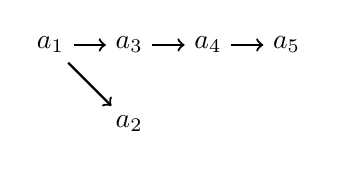
\begin{tikzpicture}
    \node(s) at (0,1) {$a_1$};
    \node(t) at (1,0) {$a_2$};
    \node(q) at (1,1) {$a_3$};
    \node(d) at (2,1) {$a_4$};
    \node(v) at (3,1) {$a_5$};
    \path[->,thick] (s) edge (q);
    \path[->,thick] (q) edge (d);
    \path[->,thick] (d) edge (v);
    \path[->,thick] (s) edge (t);
  \end{tikzpicture}
  \caption{Graphe de dépendances des alarmes}
  \label{fig:deps}
\end{figure}


Chacun de ces ensembles sera utilisé pour générer un programme simplifié ne
contenant que des alarmes ayant une relation de dépendance, évitant ainsi
d'avoir plusieurs programmes identiques en cas de dépendances mutuelles (et
réduisant le nombre d'appels à \textsc{PathCrawler}).
On remarque que si toutes les alarmes sont dépendantes, on se retrouve dans le
cas de {\em all}, et si elles sont toutes indépendantes, on se retrouve dans le
cas de {\em each}.\\


Dans notre implémentation, nous définissons une fonction calculant pour chaque
alarme, les alarmes sur lesquelles elle a un impact.
Sur notre exemple, $impacted\_stmts(\{a_1; a_2; a_3; a_4; a_5\}) =
\{\{a_2; a_3; a_4; a_5\}; \{\}; \{a_4; a_5\}; \{a_5\}; \{\}\}$.

Cette fonction nous permet de déterminer les ``alarmes finales'', qui n'ont
d'impact sur aucune autre alarme, mais peuvent avoir des dépendances mutuelles
avec d'autres alarmes finales.
Sur notre exemple, $a_2$ et $a_5$ sont des alarmes finales (sans dépendances
mutuelles).\\

Cette notion d'alarmes finales nous permet de définir une couverture minimale
des alarmes, car selon \cite{SANTE}, chaque ensemble de la couverture contient
une classe d'équivalence d'alarmes finales et leurs dépendances.
Deux alarmes finales sont dans la même classe d'équivalence si elles ont des
dépendances mutuelles.
Sur notre exemple, $min\_cover(\{a_1; a_2; a_3; a_4; a_5\}) =
\{\{a_1; a_2\}; \{a_1; a_3; a_4; a_5\}\}$.\\

Les listes obtenues par ce calcul de couverture minimale vont ensuite paramétrer
les différents {\em slicings}, on obtient un programme simplifié par liste,
paramétré par les différentes alarmes de chaque liste. \textsc{PathCrawler} est
ensuite exécuté sur chaque programme simplifié. Les résultats récupérés
permettent d'obtenir un diagnostic partiel sur chacune des alarmes du programme
simplifié. Ces diagnostics partiels sont ensuite fusionnés au sein d'une table
d'association, on obtient donc un diagnostic global sur chaque alarme.\\

Notre contribution inclut l'implémentation du calcul de la couverture minimale
et des alarmes finales, l'analyse des résultats de \textsc{PathCrawler}, la
fusion des diagnostics et la notification des résultats sur les alarmes à
\textsc{Frama-C}, qui peut les récupérer pour la consolidation du statut de
validité des propriétés du programme \cite{property-status}.\\


Dans le cas où les ensembles couvrants contiennent de nombreuses alarmes,
{\em min} hérite de l'inconvénient de l'option {\em all} : les alarmes les plus
complexes à classifier pénalisent les autres, qui peuvent ne pas être
diagnostiquées dans le temps imparti.\\

Pour corriger ce défaut, l'option {\em smart} va appliquer {\em min}
itérativement en diminuant l'ensemble des alarmes considérées à chaque
itération. Les alarmes supprimées seront des alarmes classifiées ou des alarmes
finales.\\

De cette manière, le {\em slicing} appliqué à l'itération suivante (sur
l'ensemble des alarmes privé des alarmes finales) produira un programme
simplifié plus petit. Ainsi, les alarmes qui n'ont pas été diagnostiquées à
l'itération précédente auront une chance supplémentaire de l'être, et ainsi de
suite jusqu'à ce que toutes les alarmes soient diagnostiquées ou que l'ensemble
considéré soit vide.\\

Sur l'exemple considéré plus haut, la première itération génère la
couverture minimale $\{\{a_1; a_2\}; \{a_1; a_3; a_4; a_5\}\}$. S'il reste des
alarmes non diagnostiquées, les alarmes finales ($a_2$ et $a_5$) et les alarmes
diagnostiquées ne seront plus considérées. L'itération suivante génère la
couverture $\{\{a_1; a_3; a_4\}\}$. Et ainsi de suite.
